\documentclass[11pt,a4paper]{article}
\usepackage[indonesian]{babel}
\usepackage[utf8]{inputenc}
\usepackage[T1]{fontenc}
\usepackage{geometry}
\usepackage{graphicx}
\usepackage{amsmath}
\usepackage{amssymb}
\usepackage{listings}
\usepackage{xcolor}
\usepackage{hyperref}
\usepackage{float}
\usepackage{caption}
\usepackage{subcaption}
\usepackage{algorithm}
\usepackage{algpseudocode}
\usepackage{booktabs}
\usepackage{enumitem}
\usepackage{indentfirst}

\geometry{margin=2.5cm}
\setlength{\parindent}{2.5em}
\setlist[itemize,enumerate]{listparindent=\parindent, parsep=0.35\baselineskip}

\hypersetup{
    colorlinks=true,
    linkcolor=black,
    urlcolor=blue,
}

\lstset{
    basicstyle=\ttfamily\small,
    breaklines=true,
    frame=single,
    numbers=left,
    numberstyle=\tiny\color{gray},
    keywordstyle=\color{blue},
    commentstyle=\color{green!60!black},
    stringstyle=\color{red},
    tabsize=4,
    showstringspaces=false,
    language=Go,
}

\title{
    Tugas Kecil 2: Voxelization Objek 3D menggunakan Octree \\
    \large IF2211 Strategi Algoritma \\
    \large Program Studi Teknik Informatika \\
    \large Sekolah Teknik Elektro dan Informatika \\
    \large Institut Teknologi Bandung
}
\author{
    Muhammad Iqbal Raihan (13524011) \\[0.3cm]
    Repository: \url{https://github.com/Gixgine-budi/Tucil2_13524011}
}
\date{28 Maret 2026}

\begin{document}

\maketitle
\newpage
\tableofcontents
\newpage

% ============================================================================
\section{Latar Belakang}
% ============================================================================

Dalam IF2211 Strategi Algoritma, salah satu pendekatan dasar untuk masalah besar adalah \textit{divide and conquer}: memecah masalah menjadi submasalah sejenis yang lebih kecil, menyelesaikannya, lalu menggabungkan hasil bila perlu. Tugas Kecil 2 semester II 2025/2026 meminta software yang mengonversi model 3D dalam Wavefront OBJ menjadi representasi berbasis kubus kecil (\textit{voxelization}), mirip estetika blok pada \textit{Minecraft}. Spesifikasi mensyaratkan struktur data \textit{octree} dan algoritma \textit{divide and conquer}.

Dalam konteks ini, \textit{voxelization} memetakan objek yang direpresentasikan dengan \textit{mesh} segitiga ke kumpulan \textit{voxel} berukuran seragam pada \textit{leaf depth} maksimum; hanya permukaan yang diproses: \textit{leaf} yang berpotongan dengan geometri segitiga dipertahankan sebagai \textit{voxel}, ruang kosong tidak dibelah lebih jauh. \textit{Octree} memodelkan \textit{spatial partitioning}: setiap \textit{node} adalah sel kubus; \textit{internal nodes} punya delapan anak (\textit{octants}); subdivisi 3D bersifat rekursif.

Program \texttt{ttov} ditulis dalam Go. Program membaca OBJ minimal (\texttt{v}, \texttt{f}), membangun \textit{axis-aligned bounding cube} untuk seluruh \textit{vertices}, lalu mengeksplorasi \textit{octree} sampai \textit{depth limit} dari pengguna. Hanya cabang yang masih memotong segitiga yang terus di-\textit{subdivide}; cabang kosong di-\textit{prune} lebih awal. Output berupa satu file OBJ yang berisi \textit{quad mesh} (enam \textit{quads} per \textit{voxel}) dengan \textit{vertex deduplication}, ditulis ke \texttt{output4.obj} di \textit{working directory}. Tugas dikerjakan secara individu tanpa pembagian tugas: \textit{design}, \textit{implementation}, \textit{testing}, dan laporan menjadi tanggung jawab penulis.

% ============================================================================
\section{Dasar Teori}
% ============================================================================

\subsection{\textit{Divide and conquer}}

\textit{Divide and conquer} adalah strategi algoritmik di mana suatu masalah dibagi menjadi satu atau beberapa kasus sejenis yang lebih kecil, setiap kasus diselesaikan, lalu hasilnya digabungkan. Kompleksitas sering membaik bila kasus saling independen dan ukuran masalah turun secara signifikan pada tiap pembagian; pada banyak masalah geometri, pembagian yang cerdas juga memungkinkan membuang seluruh cabang yang tidak relevan tanpa menghitung solusi parsialnya.

Pada \textit{voxelization} berbasis ruang 3D, masalah induk dapat dipandang sebagai sel kubus awal yang mencakup \textit{mesh}. Langkah \textit{divide}: jika sel berpotongan dengan segitiga dan belum mencapai kedalaman batas, sel dipecah menjadi delapan subruang yang sama besar. Tiap subruang membawa subset segitiga yang mungkin memotong subruang tersebut (\textit{culling}), sehingga submasalah lebih kecil baik secara geometri maupun jumlah segitiga. Jika sel tidak berpotongan dengan segitiga sama sekali, cabang di bawahnya tidak perlu dibangun (\textit{pruning}). Langkah \textit{conquer}: pada kedalaman maksimum, setiap sel yang masih berpotongan dengan segitiga ditetapkan sebagai \textit{voxel} permukaan. Penggabungan hasil pada akhirnya berupa pengumpulan daun yang terisi.

Struktur data yang memfasilitasi pembagian delapan arah ini adalah \textit{octree}: setiap \textit{node} menyimpan sel kubus \textit{axis-aligned}; \textit{internal node} memiliki hingga delapan anak (\textit{octants}); tiap level membagi panjang rusuk menjadi setengah sehingga volume tiap anak seperdelapan dari induk. \textit{Octree} bukan algoritma tersendiri melainkan kerangka spasial tempat langkah \textit{divide} dan \textit{prune} dijalankan secara terstruktur.

\subsection{Deteksi \textit{collision} antara \textit{voxel} dan muka segitiga}

Setiap keputusan subdivisi dan penandaan \textit{leaf} bergantung pada kondisi apakah kubus sel (\textit{voxel}, model sebagai \textit{AABB}) berpotongan dengan muka segitiga. Pada implementasi, jawaban ini dihitung sebagai rangkaian tes bertingkat, dimulai dengan pengecekan AABB, diikuti dengan pengecekan berbasis \textit{separating axis theorem} (SAT).

\subsubsection{Tes \textit{AABB} pada sumbu kartesian}

\textit{Axis-aligned bounding box} (\textit{AABB}) kubus sel sejajar dengan sumbu $x$, $y$, dan $z$. Segitiga juga dibungkus \textit{AABB} dari ketiga titik sudutnya. Dua \textit{AABB} tidak mungkin berpotongan jika pada salah satu sumbu interval proyeksi keduanya terpisah.

\subsubsection{Straddle terhadap bidang segitiga}

Segitiga membentuk bidang dengan normal $\mathbf{n} = (\mathbf{b}-\mathbf{a}) \times (\mathbf{c}-\mathbf{a})$ untuk sudut $\mathbf{a},\mathbf{b},\mathbf{c}$. Untuk tiap sudut kubus dihitung nilai yang setara dengan jarak bertanda ke bidang melalui $\mathbf{a}$. Jika semua nilai bertanda tidak berubah tanda (semua tidak negatif atau semua tidak positif tanpa melintasi nol), seluruh kubus terletak di satu sisi bidang sehingga tidak memotong segitiga. Jika ada perubahan tanda, kubus memotong bidang tak-hingga yang dibentuk oleh segitiga, sehingga pasangan tetap menjadi kandidat dan dilanjutkan ke tahap SAT.

\subsubsection{\textit{Separating axis theorem} (SAT)}

Untuk dua himpunan konveks di $\mathbb{R}^3$, keduanya terpisah (tanpa overlap volume interior) jika terdapat sumbu sedemikian sehingga proyeksi ortogonal keduanya ke sumbu itu berupa dua interval yang tidak overlap. Jika tidak ditemukan sumbu pemisah dalam himpunan sumbu uji yang memadai, untuk pasangan segitiga versus \textit{AABB} disimpulkan ada overlap. Teorema ini disebut \textit{separating axis theorem} (SAT).

Himpunan sumbu uji untuk segitiga dan \textit{AABB} mencakup arah yang relevan dengan normal bidang (telah tercakup oleh tes straddle), vektor rusuk yang sejajar sumbu kubus, dan sumbu dari \textit{cross product} $\mathbf{e}_{\triangle} \times \mathbf{d}_{\text{kubus}}$ dengan $\mathbf{e}_{\triangle}$ vektor sisi segitiga dan $\mathbf{d}_{\text{kubus}}$ vektor rusuk kubus. Pada tiap sumbu yang tidak \textit{degenerate} (bukan vektor nol), titik sudut kubus dan titik sudut segitiga diproyeksikan lewat \textit{dot product}; diperoleh interval $[\min,\max]$ untuk masing-masing bentuk. Jika $\max_{\text{kubus}} \leq \min_{\triangle}$ atau $\min_{\text{kubus}} \geq \max_{\triangle}$, sumbu tersebut memisahkan keduanya. Pada implementasi ini, kontak \textit{touching-only} (tepat pada batas interval) tidak dianggap sebagai tabrakan. Setelah semua sumbu diuji tanpa pemisah, disimpulkan ada perpotongan. Rangkaian tes keseluruhan adalah \textit{AABB}, straddle bidang, lalu loop SAT pada sumbu hasil \textit{cross product} sisi segitiga dengan rusuk kubus.

\subsection{Konkurensi dan paralelisasi}

Konkurensi berarti beberapa alur eksekusi (\textit{threads}, \textit{goroutine}, atau proses) berjalan bersamaan dalam satu periode waktu; pada CPU multi-\textit{core}, bagian pekerjaan yang independen dapat dijadwalkan paralel sehingga wall-clock time berkurang. Syarat utamanya adalah minimnya ketergantungan data serta perlindungan penulisan bersama (misalnya dengan \texttt{mutex}), karena \textit{data race} merusak konsistensi pohon atau struktur antrean.

Pada eksplorasi \textit{octree}, submasalah yang bersesuaian dengan \textit{octant} berbeda di level atas saling independen asalkan masing-masing menerima salinan atau referensi aman ke data segitiga yang sudah disaring. Oleh karena itu delapan cabang pertama dapat diluncurkan sebagai tugas konkuren terpisah. Namun jumlah tugas yang dapat dijadwalkan efisien terbatas; jika \textit{goroutine} yang aktif jauh melebihi jumlah \textit{logical core}, biaya \textit{scheduling} dan \textit{stack} meningkat. Pola mitigasi yang dipakai program adalah ketika jumlah \textit{goroutine} aktif melampaui kira-kira dua kali \texttt{GOMAXPROCS}, pembangunan \textit{subtree} dilanjutkan secara iteratif dengan \textit{breadth-first queue}, yang tetap benar secara semantik tetapi membatasi ledakan konkurensi.

% ============================================================================
\section{Implementasi Algoritma}
% ============================================================================

\subsection{\textit{Divide and conquer}}

Secara konseptual, pipeline berikut menjelaskan apa yang dilakukan tiap tahap sebelum masuk ke detail tipe data dan fungsi, dari \textit{mesh} segitiga yang valid sampai \textit{file} OBJ berisi \textit{voxel}. Urutan ini mengikuti pola \textit{divide and conquer} pada ruang 3D, yaitu menyaring geometri yang relevan lalu memecah sel hanya bila masih ada perpotongan dengan segitiga.

\begin{enumerate}[leftmargin=*, itemsep=0.75\baselineskip]
    \item Memvalidasi dan memuat \textit{mesh}.

    Program membaca baris \texttt{v} dan \texttt{f}, menolak format yang tidak sesuai, lalu menyusun \textit{vertex list} dan \textit{triangle list} sebagai satu-satunya sumber geometri untuk tahap berikutnya.

    \item Menentukan kubus pembatas \textit{axis-aligned}.

    Dibangun kubus terkecil sejajar sumbu yang mencakup semua \textit{vertices}. Panjang rusuk diambil sebagai $\max$ dari rentang $x$, $y$, dan $z$ agar domain subdivisi berbentuk kubus, bukan balok sembarang.

    \item \textit{Subdivide} dan \textit{cull} segitiga untuk tiap sel.

    Kubus besar dipecah menjadi delapan \textit{octants}, setiap sel diuji interseksinya dengan segitiga, dan hanya subset segitiga yang benar-benar memotong \textit{child cell} yang dibawa ke level berikutnya hingga \textit{depth limit}. Sel yang kosong tidak dibelah lagi sehingga biaya komputasi tetap terkendali.

    \item Menandai \textit{surface voxel} pada kedalaman maksimum.

    Pada batas kedalaman, setiap sel yang masih berpotongan dengan segitiga ditandai sebagai \textit{voxel} permukaan.

    \item Mengekspor OBJ dengan \textit{vertex deduplication}.

    Kumpulan kubus diubah menjadi baris \texttt{v} dan \texttt{f} pada format OBJ (\textit{quads}), kemudian \textit{vertices} pada posisi yang sama digabung agar ukuran berkas tidak terlalu besar akibat titik duplikat di sisi antar-\textit{voxel} yang bersebelahan.
\end{enumerate}

\subsection{Representasi data}

Tipe utama: \texttt{vertex} untuk titik 3D; \texttt{face} untuk segitiga berindeks ke \texttt{objFile.vertices}; \texttt{voxel} sebagai kubus (\texttt{base}, \texttt{size}); \texttt{octree} sebagai \textit{tree node} dengan pointer \texttt{voxel}, \texttt{depth}, flag \texttt{fill}, delapan anak. Output voxel: \texttt{objFile4} berisi \texttt{face4} (\textit{quads}).

\begin{lstlisting}[caption={Core types (struct.go)}]
type objFile struct {
    vertices []vertex
    faces    []face
}

type octree struct {
    size     float64
    root     *voxel
    depth    int
    fill     bool
    children [8]*octree
}
\end{lstlisting}

\subsection{Alur utama}

\begin{algorithm}[H]
\caption{Octree-based voxelization (outline)}
\begin{algorithmic}[1]
\Require Valid triangle OBJ file, non-negative integer $L$ (\textit{subdivision depth limit})
\Ensure File \texttt{output4.obj} with \textit{surface voxels} as axis-aligned cubes
\State Parse and validate \texttt{v} and \texttt{f} lines
\State Compute \textit{bounding cube} covering all vertices
\State Build \textit{octree}: eight top-level \textit{octants} in parallel, then recursive/iterative per node
\State At depth $L$, mark leaves intersecting triangles as voxels
\State Emit filled leaves as quads, dedupe vertices, write OBJ
\end{algorithmic}
\end{algorithm}

\subsection{\textit{Octree} subdivision and exploration}

\texttt{voxel.subdivide} memecah sel menjadi delapan kubus dengan \textit{edge length} setengahnya. \texttt{exploreObj} membuat akar dan menjalankan eksplorasi untuk delapan anak \textit{world cube}. Rutin paralel menyaring segitiga yang \textit{collide} dengan sel saat ini. Tanpa segitiga, \textit{node} kosong dan tanpa anak. Pada \textit{depth limit}, \texttt{fill} ditentukan berdasarkan apakah masih ada interseksi dengan segitiga (\textit{surface voxel}). Sebelum mencapai \textit{depth limit}, jika masih ada segitiga, delapan anak dibangun dengan subset yang sudah di-\textit{cull}.

\subsection{Rutin \textit{collision} (\texttt{checkCollision})}

\texttt{checkCollision} mengimplementasikan tes interseksi antara \textit{voxel} dan segitiga: AABB, bidang, lalu SAT pada \textit{edges}. Jika ada \textit{separating axis}, mengembalikan \texttt{false} (no intersection).

\subsection{Ekspor OBJ dan statistik}

\texttt{octToObj} melakukan \textit{BFS traversal} untuk menghitung \textit{nodes} per \textit{depth}, perkiraan \textit{nodes not explored} pada level berikutnya ketika cabang kosong, dan jumlah \textit{leaf voxels} yang ditulis. \texttt{compactObj4} menggabungkan \textit{vertices} identik.

\subsection{I/O dan pelaporan CLI}

Input interaktif dari \textit{standard input}: path file OBJ, lalu \textit{subdivision level} (berapa kali kubus dipecah menjadi delapan; contoh pada program: level 3 $\Rightarrow$ hingga $8^3$ \textit{finest cells} sepanjang satu jalur penuh). Program mencetak waktu untuk OBJ \textit{scan}, voxelization, konversi ke struktur OBJ, \textit{compaction}, dan \textit{write}, plus waktu total. Juga jumlah \textit{voxels}, \textit{vertices}, \textit{faces} setelah \textit{compaction}, tabel \textit{nodes per depth}, tabel \textit{nodes not explored per depth}. Output file: \texttt{output4.obj} di \textit{working directory}.

Validasi OBJ: wajib \texttt{v} dengan tiga koordinat dan \texttt{f} dengan tiga indeks segitiga (1-based di file); baris yang diawali \texttt{\#} diabaikan; tipe baris yang tidak dikenal $\Rightarrow$ error.

% ============================================================================
\section{Analisis Kompleksitas}
% ============================================================================

\subsection{Kompleksitas waktu}

Misalkan $F$ jumlah segitiga input dan $L$ \textit{depth limit}. Per \textit{node}, pada kasus terburuk semua segitiga yang dibawa ikut diuji terhadap sel; biaya per pasangan bersifat konstan (ditentukan oleh rutin interseksi geometri). \textit{Tree} pada kasus terlebar memiliki $\sim8^L$ \textit{leaves}, namun \textit{pruning} sel kosong mengurangi \textit{nodes} yang dibangun untuk \textit{mesh} yang tidak memenuhi seluruh ruang. Tanpa \textit{pruning}, waktu kasus terburuk bersifat eksponensial terhadap $L$ dan bergantung secara linear terhadap $F$. Pada praktiknya jumlah \textit{nodes} jauh lebih kecil, tercermin pada kolom \textit{nodes not explored} di keluaran program.

\subsection{Kompleksitas ruang}

Penyimpanan \textit{tree} sebanding dengan jumlah \textit{nodes} yang dialokasi; mode iteratif menyimpan \textit{frontier queue}. Output menyimpan $O(V)$ \textit{vertices} unik dan $O(V)$ \textit{quads} untuk $V$ \textit{leaf voxels} sebelum \textit{compaction}, berkurang setelah \textit{deduplication} antarkubus yang berbagi sisi.

% ============================================================================
\section{Pengujian}
% ============================================================================

Spesifikasi mensyaratkan screenshot input dan output program untuk setidaknya lima contoh berbeda. Lingkungan uji: \texttt{go 1.26.1}, AMD Ryzen 7 7435HS, Windows 11.

\subsection{Kasus uji}

\subsubsection{Kasus uji 1}

\begin{itemize}[leftmargin=*, itemsep=0.75\baselineskip, topsep=0.5\baselineskip]
    \item Input

    OBJ path: \texttt{test/cow.obj}, \textit{subdivision level}: $8$.

    \item Expected behavior

    Program menulis \texttt{output4.obj} dan mencetak jumlah \textit{voxel}, \textit{vertex}, dan \textit{face}, statistik \textit{node} per \textit{depth}, jumlah \textit{nodes not explored} per \textit{depth}, serta \textit{timings}.

    \item Hasil
\end{itemize}

\begin{verbatim}
    $ .\build.bat run
    Building ttov...
    Enter file path: test/cow.obj
    
    Subdivision level is the number of times the cube is subdivided into 8 smaller cubes.
    For example, a subdivision level of 3 means the cube is subdivided into 8^3 = 512 smaller cubes.
    Enter subdivision level: 8
    
    
    ============================================================
    Scanning .obj file completed
    Time taken to scan obj file: 22.3386ms
    
    Octree generation completed
    Time taken to voxelize obj file: 169.6209ms
    
    Octree to OBJ data type conversion completed
    Time taken to convert octree to OBJ data type: 124.1921ms
    
    OBJ data has been succesfully compacted
    Time taken to compact OBJ data: 343.632ms
    
    Number of voxels: 91951
    Number of vertices: 306960
    Number of faces: 551706
    
    Number of nodes at each depth:
    1       : 1
    2       : 8
    3       : 32
    4       : 152
    5       : 696
    6       : 2728
    7       : 10928
    8       : 45248
    9       : 182424
    
    Number of nodes not explored at each depth:
    1       : 0
    2       : 0
    3       : 32
    4       : 104
    5       : 520
    6       : 2840
    7       : 10896
    8       : 42176
    9       : 179560
    
    
    OBJ file writing completed
    Time taken to write obj file: 183.0416ms
    
    Total time taken: 842.8252ms
\end{verbatim}

\begin{figure}[H]
    \centering
    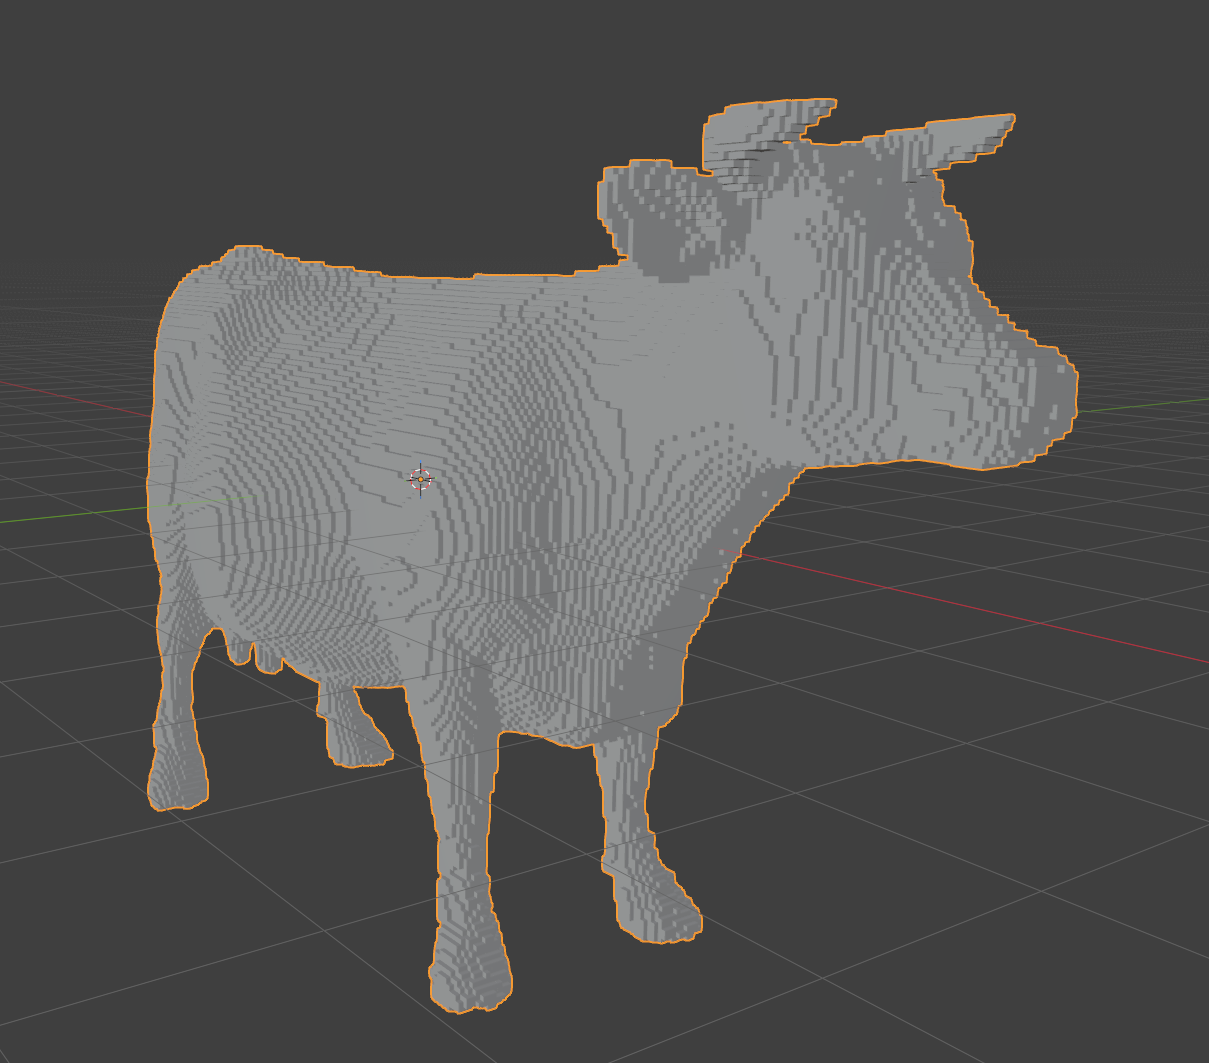
\includegraphics[width=0.75\textwidth]{img/test1.png}
    \caption{Test case 1}
\end{figure}

\subsubsection{Kasus uji 2}
\begin{itemize}[leftmargin=*, itemsep=0.75\baselineskip, topsep=0.5\baselineskip]
    \item Input

    OBJ path: \texttt{test/pumpkin.obj}, \textit{subdivision level}: $9$.

    \item Expected behavior

    Program menulis \texttt{output4.obj} dan mencetak jumlah \textit{voxel}, \textit{vertex}, dan \textit{face}, statistik \textit{node} per \textit{depth}, jumlah \textit{nodes not explored} per \textit{depth}, serta \textit{timings}.

    \item Hasil
\end{itemize}

\begin{verbatim}
    $ .\build.bat run
    Building ttov...
    Enter file path: test/pumpkin.obj
    
    Subdivision level is the number of times the cube is subdivided into 8 smaller cubes.
    For example, a subdivision level of 3 means the cube is subdivided into 8^3 = 512 smaller cubes.
    Enter subdivision level: 9 
    
    
    ============================================================
    Scanning .obj file completed
    Time taken to scan obj file: 40.6941ms
    
    Octree generation completed
    Time taken to voxelize obj file: 832.4522ms
    
    Octree to OBJ data type conversion completed
    Time taken to convert octree to OBJ data type: 1.7177806s
    
    OBJ data has been succesfully compacted
    Time taken to compact OBJ data: 7.8247703s
    
    Number of voxels: 1196633
    Number of vertices: 3960457
    Number of faces: 7179798
    
    Number of nodes at each depth:
    1       : 1
    2       : 8
    3       : 64
    4       : 448
    5       : 2024
    6       : 8864
    7       : 36824
    8       : 148864
    9       : 596992
    10      : 2391672
    
    Number of nodes not explored at each depth:
    1       : 0
    2       : 0
    3       : 0
    4       : 64
    5       : 1560
    6       : 7328
    7       : 34088
    8       : 145728
    9       : 593920
    10      : 2384264
    
    
    OBJ file writing completed
    Time taken to write obj file: 3.5628761s
    
    Total time taken: 13.9785733s
\end{verbatim}

\begin{figure}[H]
    \centering
    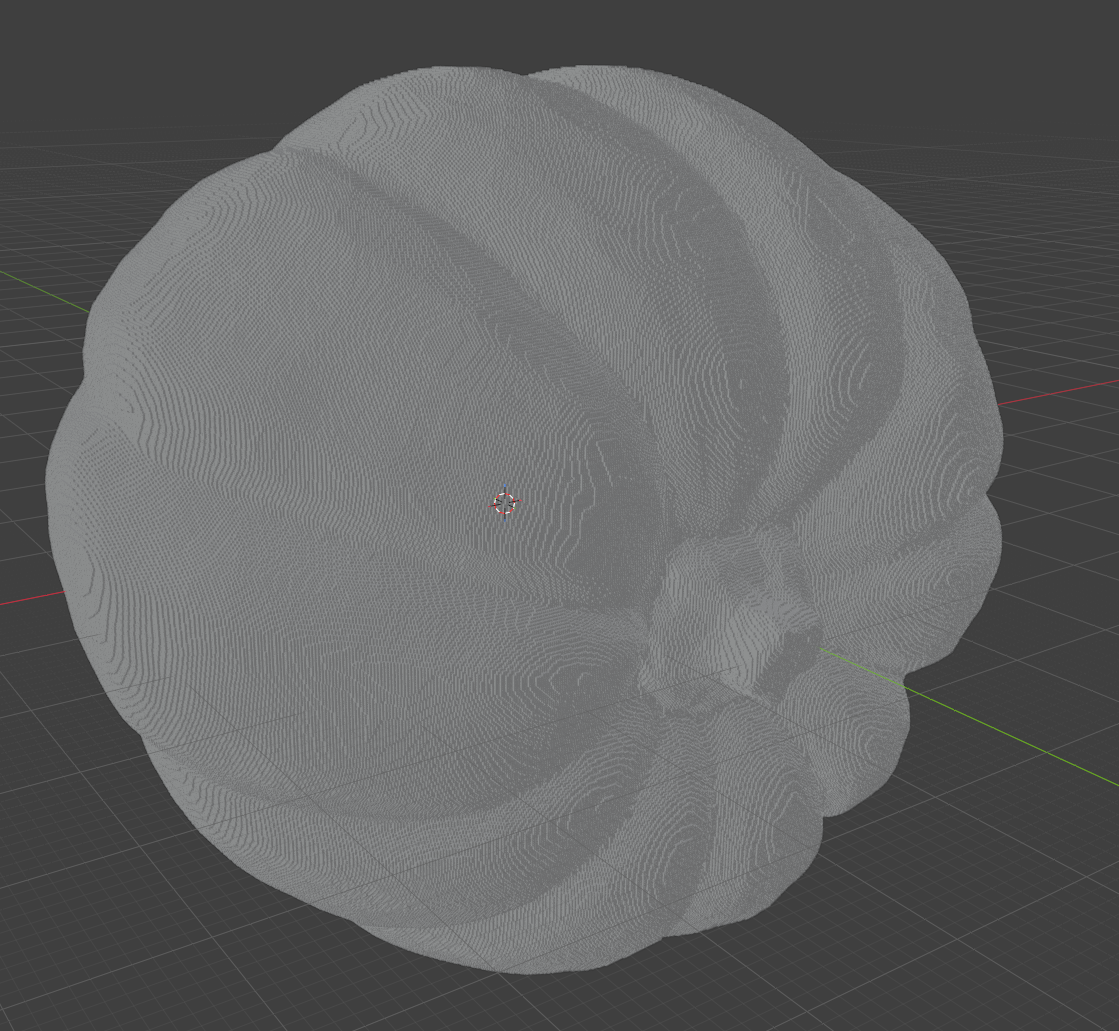
\includegraphics[width=0.75\textwidth]{img/test2.png}
    \caption{Test case 2}
\end{figure}

\subsubsection{Kasus uji 3}
\begin{itemize}[leftmargin=*, itemsep=0.75\baselineskip, topsep=0.5\baselineskip]
    \item Input

    OBJ path: \texttt{test/teapot.obj}, \textit{subdivision level}: $8$.

    \item Expected behavior

    Program menulis \texttt{output4.obj} dan mencetak jumlah \textit{voxel}, \textit{vertex}, dan \textit{face}, statistik \textit{node} per \textit{depth}, jumlah \textit{nodes not explored} per \textit{depth}, serta \textit{timings}.

    \item Hasil
\end{itemize}

\begin{verbatim}
    $ .\build.bat run
    Building ttov...
    Enter file path: test/teapot.obj
    
    Subdivision level is the number of times the cube is subdivided into 8 smaller cubes.
    For example, a subdivision level of 3 means the cube is subdivided into 8^3 = 512 smaller cubes.
    Enter subdivision level: 8
    
    
    ============================================================
    Scanning .obj file completed
    Time taken to scan obj file: 32.6059ms
    
    Octree generation completed
    Time taken to voxelize obj file: 102.9254ms
    
    Octree to OBJ data type conversion completed
    Time taken to convert octree to OBJ data type: 145.3819ms
    
    OBJ data has been succesfully compacted
    Time taken to compact OBJ data: 383.2267ms
    
    Number of voxels: 118263
    Number of vertices: 329286
    Number of faces: 709578
    
    Number of nodes at each depth:
    1       : 1
    2       : 8
    3       : 32
    4       : 160
    5       : 784
    6       : 3440
    7       : 14272
    8       : 58400
    9       : 236152
    
    Number of nodes not explored at each depth:
    1       : 0
    2       : 0
    3       : 32
    4       : 96
    5       : 496
    6       : 2832
    7       : 13248
    8       : 55776
    9       : 231048
    
    
    OBJ file writing completed
    Time taken to write obj file: 252.1601ms
    
    Total time taken: 916.3ms
\end{verbatim}

\begin{figure}[H]
    \centering
    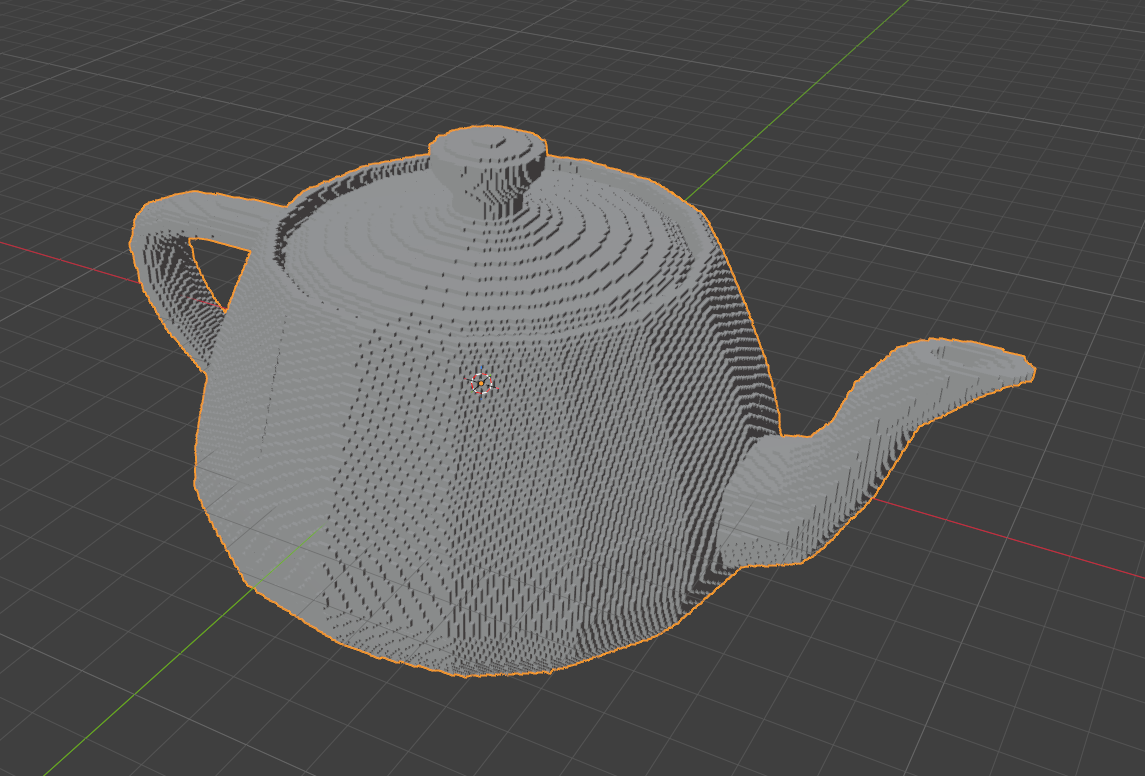
\includegraphics[width=0.75\textwidth]{img/test3.png}
    \caption{Test case 3}
\end{figure}

\subsubsection{Kasus uji 4}
\begin{itemize}[leftmargin=*, itemsep=0.75\baselineskip, topsep=0.5\baselineskip]
    \item Input

    OBJ path: \texttt{test/line.obj}, \textit{subdivision level}: $5$.

    \item Expected behavior

    Program menulis \texttt{output4.obj} dan mencetak jumlah \textit{voxel}, \textit{vertex}, dan \textit{face}, statistik \textit{node} per \textit{depth}, jumlah \textit{nodes not explored} per \textit{depth}, serta \textit{timings}.

    \item Hasil
\end{itemize}

\begin{verbatim}
    $ .\build.bat run
    Building ttov...
    Enter file path: test/line.obj
    
    Subdivision level is the number of times the cube is subdivided into 8 smaller cubes.
    For example, a subdivision level of 3 means the cube is subdivided into 8^3 = 512 smaller cubes.
    Enter subdivision level: 5
    
    
    ============================================================
    Scanning .obj file completed
    Time taken to scan obj file: 1.0979ms
    
    Octree generation completed
    Time taken to voxelize obj file: 2.7027ms
    
    Octree to OBJ data type conversion completed
    Time taken to convert octree to OBJ data type: 552.5µs
    
    OBJ data has been succesfully compacted
    Time taken to compact OBJ data: 1.0945ms
    
    Number of voxels: 288
    Number of vertices: 868
    Number of faces: 1728
    
    Number of nodes at each depth:
    1       : 1
    2       : 8
    3       : 24
    4       : 56
    5       : 216
    6       : 672
    
    Number of nodes not explored at each depth:
    1       : 0
    2       : 0
    3       : 40
    4       : 136
    5       : 232
    6       : 1056
    
    
    OBJ file writing completed
    Time taken to write obj file: 7.3778ms
    
    Total time taken: 12.8254ms
\end{verbatim}

\begin{figure}[H]
    \centering
    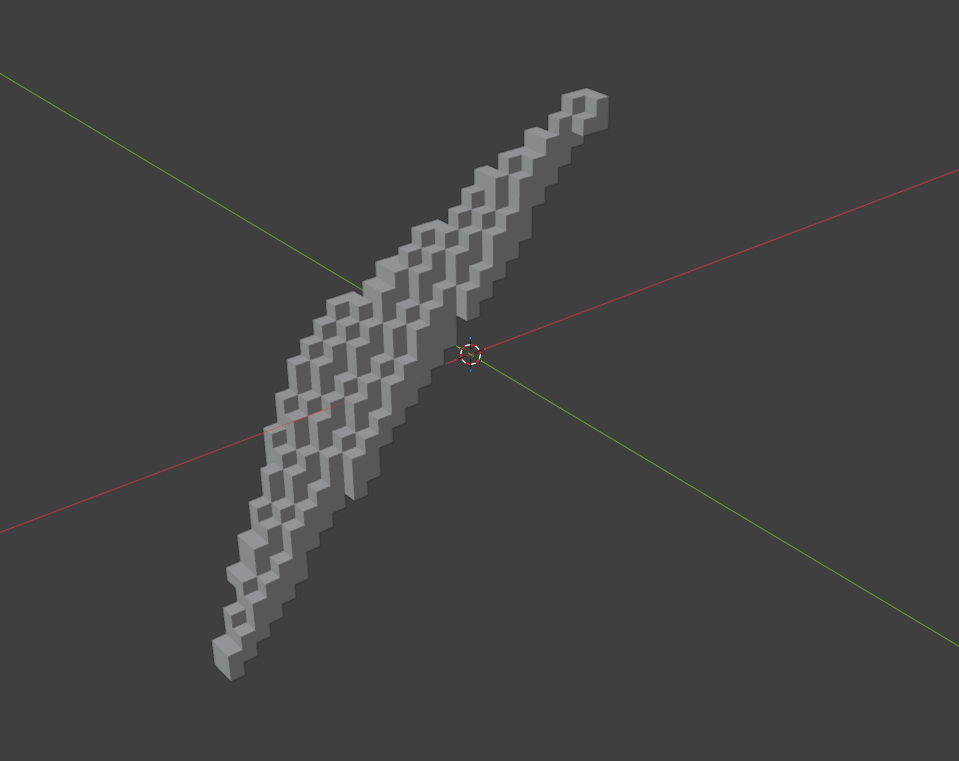
\includegraphics[width=0.75\textwidth]{img/test4.png}
    \caption{Test case 4}
\end{figure}

\subsubsection{Kasus uji 5}
\begin{itemize}[leftmargin=*, itemsep=0.75\baselineskip, topsep=0.5\baselineskip]
    \item Input

    OBJ path: \texttt{test/chen.obj}, \textit{subdivision level}: $10$.

    \item Expected behavior

    Program menulis \texttt{output4.obj} dan mencetak jumlah \textit{voxel}, \textit{vertex}, dan \textit{face}, statistik \textit{node} per \textit{depth}, jumlah \textit{nodes not explored} per \textit{depth}, serta \textit{timings}.

    \item Hasil
\end{itemize}

\begin{verbatim}
    $ .\build.bat run
    Building ttov...
    Enter file path: test/chen.obj
    
    Subdivision level is the number of times the cube is subdivided into 8 smaller cubes.
    For example, a subdivision level of 3 means the cube is subdivided into 8^3 = 512 smaller cubes.
    Enter subdivision level: 10
    
    
    ============================================================
    Scanning .obj file completed
    Time taken to scan obj file: 131.023ms
    
    Octree generation completed
    Time taken to voxelize obj file: 2.3589979s
    
    Octree to OBJ data type conversion completed
    Time taken to convert octree to OBJ data type: 2.7613098s
    
    OBJ data has been succesfully compacted
    Time taken to compact OBJ data: 7.1535419s
    
    Number of voxels: 1789487
    Number of vertices: 5026538
    Number of faces: 10736922
    
    Number of nodes at each depth:
    1       : 1
    2       : 8
    3       : 24
    4       : 112
    5       : 472
    6       : 1856
    7       : 8320
    8       : 35240
    9       : 158976
    10      : 724192
    11      : 3254280
    
    Number of nodes not explored at each depth:
    1       : 0
    2       : 0
    3       : 40
    4       : 80
    5       : 424
    6       : 1920
    7       : 6528
    8       : 31320
    9       : 122944
    10      : 547616
    11      : 2539256
    
    
    OBJ file writing completed
    Time taken to write obj file: 3.1406528s
    
    Total time taken: 15.5455254s
\end{verbatim}

\begin{figure}[H]
    \centering
    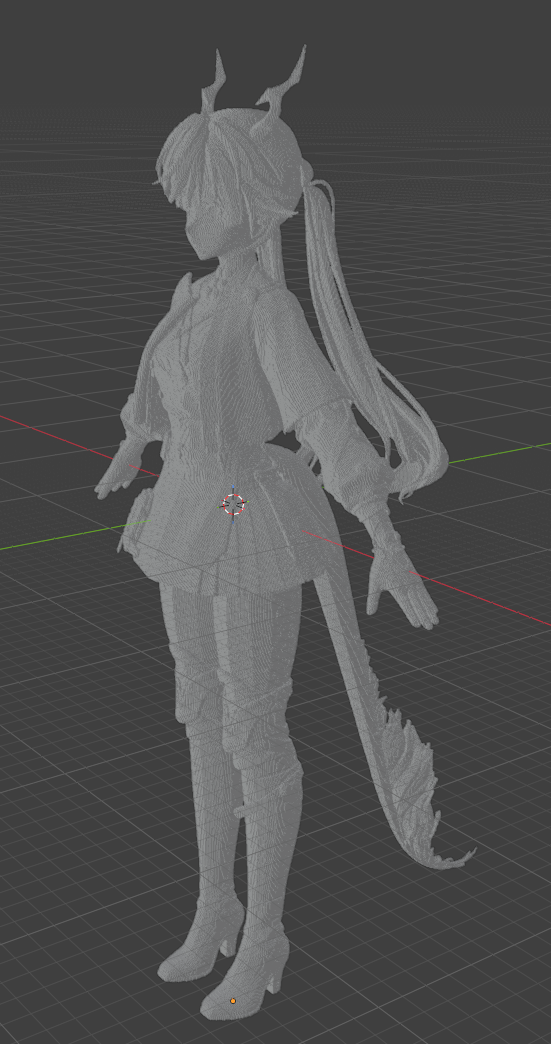
\includegraphics[width=0.75\textwidth]{img/test5.png}
    \caption{Test case 5}
\end{figure}

\subsection{Ringkasan hasil pengujian}

\begin{table}[H]
\centering
\begin{tabular}{@{}clccrl@{}}
\toprule
No. & File / scenario & Level $L$ & Total time & Voxels & Notes \\
\midrule
1 & \texttt{test/cow.obj} & 8 & 0{,}843 s & 91\,951 & Stanford Cow \\
2 & \texttt{test/pumpkin.obj} & 9 & 13{,}98 s & 1\,196\,633 & \\
3 & \texttt{test/teapot.obj} & 8 & 0{,}916 s & 118\,263 & \\
4 & \texttt{test/line.obj} & 5 & 0{,}013 s & 288 &  \\
5 & \texttt{test/chen.obj} & 10 & 15{,}55 s & 1\,789\,487 & Chen Qianyu \\
\bottomrule
\end{tabular}
\caption{Ringkasan lima kasus uji}
\end{table}

% ============================================================================
\section{Kesimpulan}
% ============================================================================

Program \texttt{ttov} yang ditulis dalam Go melakukan voxelization OBJ segitiga dengan \textit{octree} dan \textit{divide and conquer}, \textit{pruning} cabang kosong, dan eksplorasi paralel di level atas. \texttt{output4.obj} berisi \textit{surface voxels} dengan \textit{uniform cube size} pada \textit{max depth}, sesuai dengan spesifikasi I/O dan pelaporan statistik di CLI. Keterbatasan utama: ukuran file keluaran dan waktu komputasi membesar untuk \textit{mesh} yang sangat padat atau $L$ yang besar, serta asumsi OBJ minimal. Pengembangan lebih lanjut dapat berupa perapihan metrik \textit{depth} di output teks atau heuristik untuk mengurangi uji segitiga per sel.

% ============================================================================
\appendix
\section{Checklist penilaian}
% ============================================================================

\begin{table}[H]
\centering
\begin{tabular}{@{}clcc@{}}
\toprule
No. & Poin & Ya & Tidak \\
\midrule
1 & Program berhasil dikompilasi tanpa kesalahan & \checkmark & \\
2 & Program berhasil dijalankan & \checkmark & \\
3 & Hasil konversi OBJ terdiri dari kubus-kubus kecil & \checkmark & \\
4 & Program menampilkan informasi atau laporan sesuai spesifikasi & \checkmark & \\
5 & Program dapat menerima masukan OBJ dan menghasilkan keluaran & \checkmark & \\
6 & {[Bonus]} Program menggunakan konkurensi & \checkmark & \\
7 & [Bonus] Program dapat menampilkan visualisasi .obj &  & \checkmark \\
\bottomrule
\end{tabular}
\end{table}

\noindent Catatan: \textit{build} diuji pada Windows (\texttt{build.bat}) dan Linux (\texttt{Makefile}).

\end{document}
